\documentclass{article}

\usepackage{tabularx}
\usepackage{booktabs}
\usepackage[x11names]{xcolor}
\usepackage{hyperref}
\usepackage{amssymb}
\usepackage{float}
\usepackage{longtable}
\usepackage{xr}
\usepackage{graphicx}
\usepackage{cite}

\externaldocument[MG-]{../Design/SoftArchitecture/MG}
\externaldocument[SRS-]{../SRS/SRS}
\externaldocument[Hardware-]{../Extras/Hardware/HardwareReport}

\title{Reflection and Traceability Report on \progname}

\author{\authname}

\date{}

\input{../Comments}
\input{../Common}

\begin{document}

\maketitle

\section{Changes in Response to Feedback}

\plt{Summarize the changes made over the course of the project in response to
feedback from TAs, the instructor, teammates, other teams, the project
supervisor (if present), and from user testers.}

\plt{For those teams with an external supervisor, please highlight how the feedback 
from the supervisor shaped your project.  In particular, you should highlight the 
supervisor's response to your Rev 0 demonstration to them.}

\plt{Version control can make the summary relatively easy, if you used issues
and meaningful commits.  If you feedback is in an issue, and you responded in
the issue tracker, you can point to the issue as part of explaining your
changes.  If addressing the issue required changes to code or documentation, you
can point to the specific commit that made the changes.  Although the links are
helpful for the details, you should include a label for each item of feedback so
that the reader has an idea of what each item is about without the need to click
on everything to find out.}

\plt{If you were not organized with your commits, traceability between feedback
and commits will not be feasible to capture after the fact.  You will instead
need to spend time writing down a summary of the changes made in response to
each item of feedback.}

\plt{You should address EVERY item of feedback.  A table or itemized list is
recommended.  You should record every item of feedback, along with the source of
that feedback and the change you made in response to that feedback.  The
response can be a change to your documentation, code, or development process.
The response can also be the reason why no changes were made in response to the
feedback.  To make this information manageable, you will record the feedback and
response separately for each deliverable in the sections that follow.}

\plt{If the feedback is general or incomplete, the TA (or instructor) will not
be able to grade your response to feedback.  In that case your grade on this
document, and likely the Revision 1 versions of the other documents will be
low.} 

\subsection{SRS and Hazard Analysis}

\subsection{Design and Design Documentation}

\subsection{VnV Plan and Report}

\section{Extras}

The team produced two supplementary extras reports. The first focuses on the
theoretical foundations of the software algorithms used in the project,
including the Direction of Arrival algorithm and audio classification. It
explains how these algorithms were developed and validated without physical
hardware by leveraging a Python based microphone room simulation library. The
report further details the process of experimentation, refinement, and eventual
selection of algorithms for deployment on the microcontroller. The report is
located in
\href{https://github.com/Team6-SixSense/audio360/blob/main/docs/Extras/Software/SoftwareReport.pdf}
{docs/Extras/Hardware/SoftwareReport.pdf}

The second supplementary report documents the hardware used in the project. It
outlines the theory behind of key hardware components as well as some of their 
specification. It also explains how knowing the hardware theory helped supported
and constrained software design decisions. The report is located in
\href{https://github.com/Team6-SixSense/audio360/blob/main/docs/Extras/Hardware/HardwareReport.pdf}
{docs/Extras/Hardware/HardwareReport.pdf}

\section{Design Iteration (LO11 (PrototypeIterate))}

The final design was reached through an iterative process driven by hardware
readiness, user feedback, and alignment with the secondary stakeholder needs.
In the initial implementation presented at the Proof of Concept demo, the
software algorithms (Direction of Arrival and audio classification) were
developed entirely in a simulated environment using a Python microphone room
simulation library. This approach was chosen because the hardware platform was
not yet stable enough for reliable development. Simulation enabled rapid
experimentation, validation of algorithm feasibility, and early performance
comparisons of different implementations without being constrained by incomplete
hardware. On the hardware side, the system consisted of four microphones
connected to a microcontroller, capable of synchronous audio sampling,
figure \ref{fig:hardware_before}.
While this setup demonstrated that individual software and hardware components
worked as expected, it did not yet meet the stakeholder's need for an
integrated, usable system.

\begin{figure}[H]
    \centering
    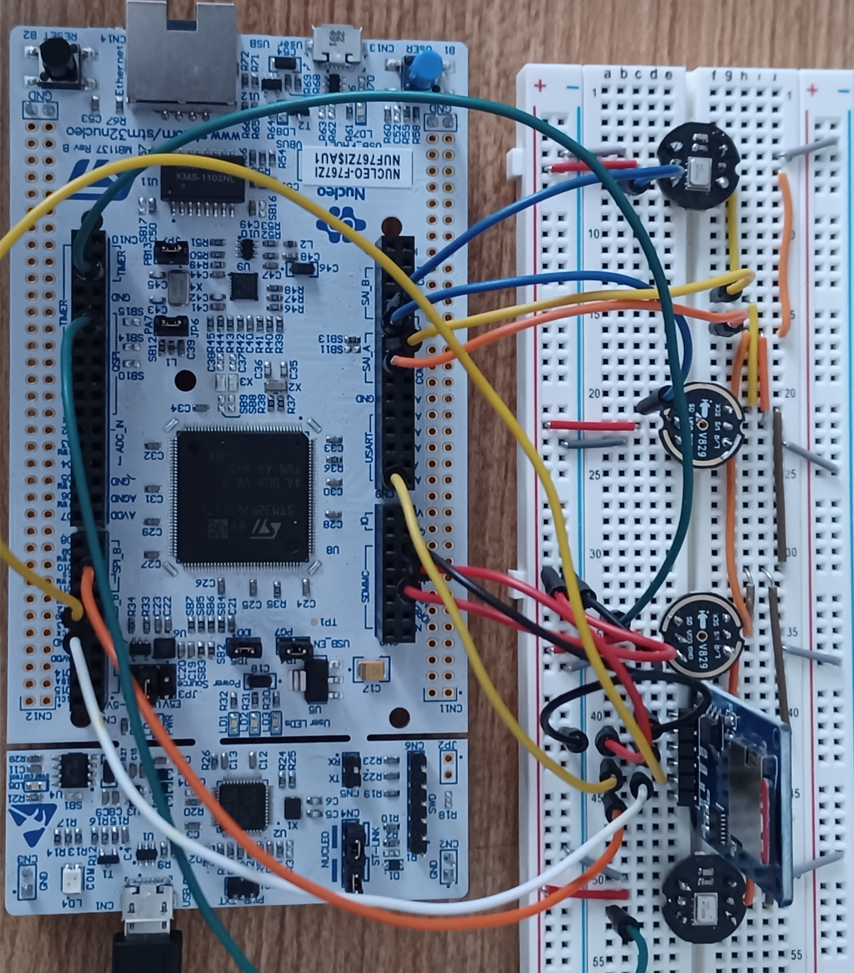
\includegraphics[width=0.5\textwidth]{./images/hardware_before.png}
    \caption{Hardware set-up for Proof of Concept.}
    \label{fig:hardware_before}
\end{figure}

As development progressed, the design evolved toward full system integration.
The software was migrated from Python to C/C++ to be compiled onto the
microcontroller. In parallel, the hardware underwent significant refinements,
including improved microphones, more reliable wiring, the addition of bluetooth
connectivity, and eventual integration into a custom PCB, figure
\ref{fig:hardware_after}. A key design decision
that enabled this parallel evolution was the adoption of a layered software
architecture. By decoupling hardware and software components, the team was able
to continue developing and testing algorithms independently of hardware
readiness using mocks in unit tests. This reduced integration risk and ensured
continuous progress toward a deployable system.


\begin{figure}[H]
    \centering
    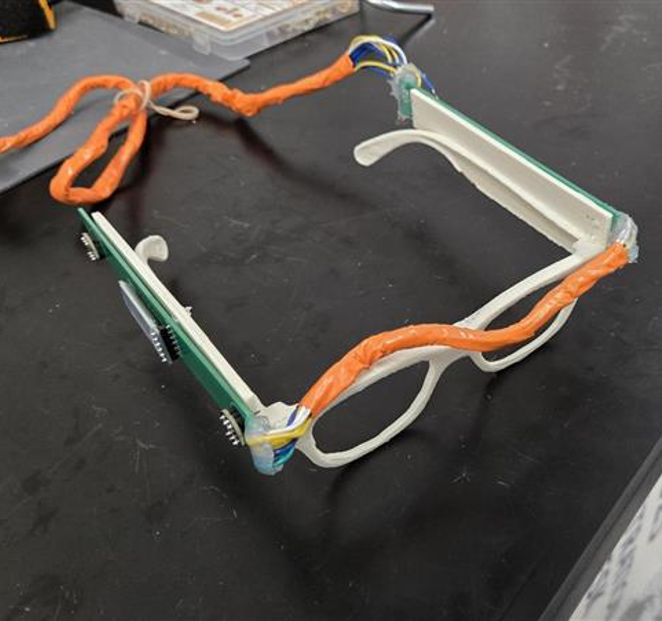
\includegraphics[width=0.5\textwidth]{./images/hardware_after.png}
    \caption{Final hardware.}
    \label{fig:hardware_after}
\end{figure}

The user interface design was also refined based on usability considerations.
The primary stakeholders are individuals who are hard of hearing. Although
direct testing with this group was not feasible, secondary stakeholders
(e.x. individuals wearing earplugs or headphones) were asked to participate in
user testing. Early UI designs were found to be overly intrusive, presenting
excessive information that interfered with users' daily activities, figure
\ref{fig:ui_before}. This violates the non-functional requirement for a
non-intrusive display, \hyperref[SRS-NFR6_2]{NFR6.2}. As a result, the
interface was simplified to present only essential information
in a less disruptive manner, figure \ref{fig:ui_after}.

\begin{figure}[H]
    \centering
    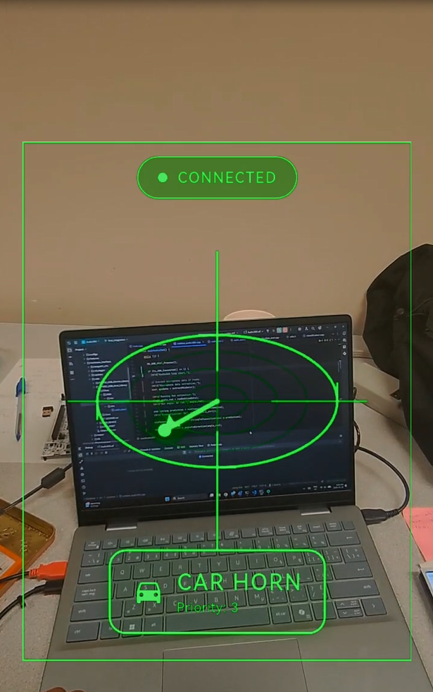
\includegraphics[width=0.5\textwidth]{./images/ui_before.png}
    \caption{Initial UI before user testing.}
    \label{fig:ui_before}
\end{figure}

\begin{figure}[H]
    \centering
    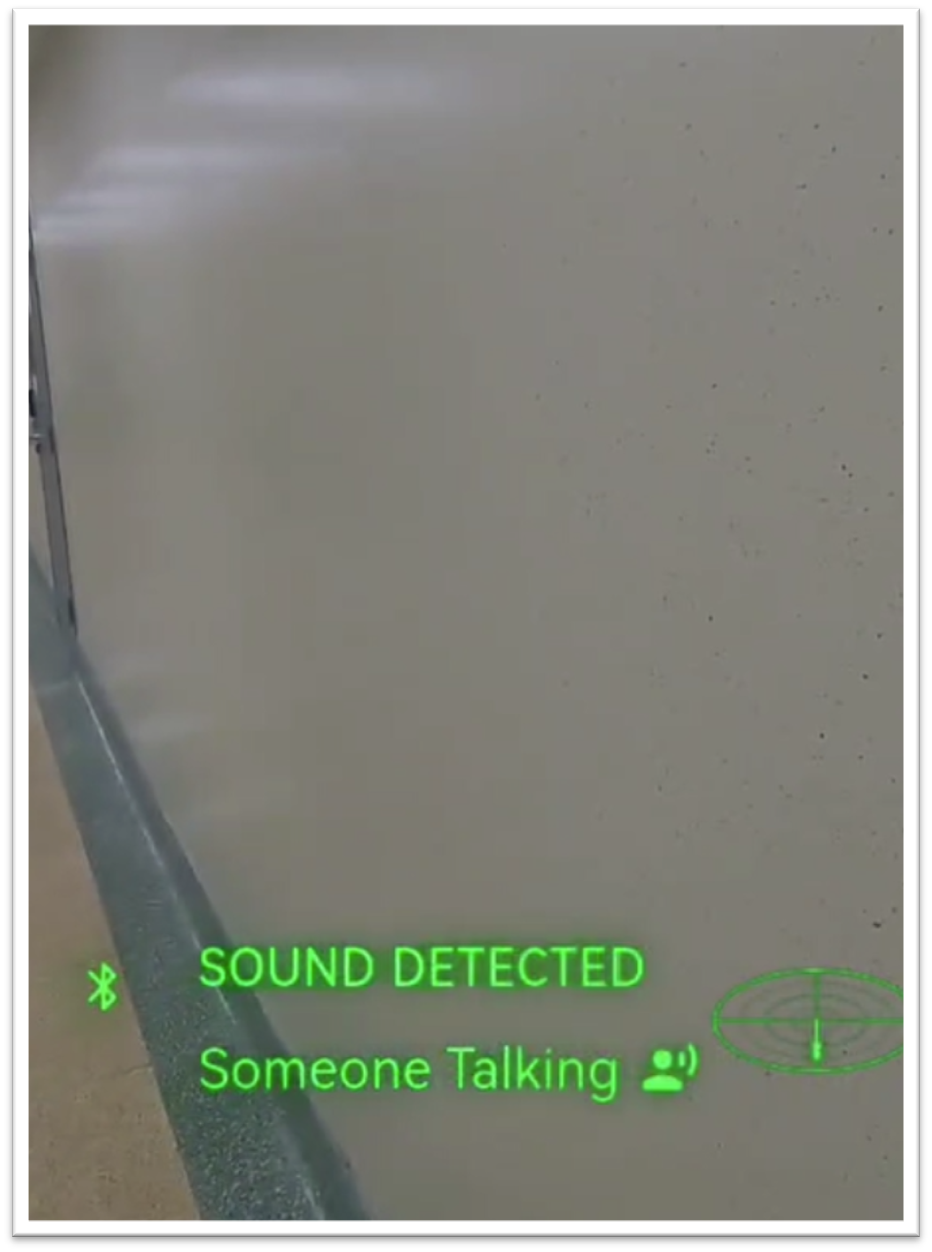
\includegraphics[width=0.5\textwidth]{./images/ui_after.png}
    \caption{UI after user testing.}
    \label{fig:ui_after}
\end{figure}

Finally, the audio classification component was refined to better reflect
meaningful real world use cases. The initial version classified sounds such as
car horns, jackhammers, and sirens. However, both user feedback and team
evaluation indicated that some of these sounds were less relevant to the core
goal of improving situational awareness. The classification categories were
therefore updated to include sirens, fire alarms, and human talking, which are
more critical for safety and everyday awareness. This required retraining and
modifying the classification module, but resulted in a system that better
serves the stakeholders' priorities.


\section{Design Decisions (LO12)}

\subsection{Limitations}

The primary limitation of the system was the restricted computational power and
memory capacity of the microcontroller. These limitations required careful
management of memory allocation and algorithmic complexity to ensure real time
performance without any faults. As a result, the team selected lightweight and
efficient algorithms. For Direction of Arrival, the GCC-PHAT algorithm was
chosen due to its relatively low computational complexity, $O(N*log(N))$, and
suitability for embedded systems. More complex alternatives were avoided as they
would exceed available resources. Similarly, the audio classification module
was limited to three classes to remain within memory constraints. This excluded
more advanced approaches, such as neural networks, which would require
significantly more memory and processing power than the platform could support.

\subsection{Constriants}

Several constraints from the SRS \cite{SRS} significantly influenced the design.
\hyperref[SRS-NFR9_1]{NFR9.1} specified that the system must operate as
a closed system, meaning no external devices or services could be used.
This constraint was motivated by security considerations. As a result, this
constraint eliminated the possibility of offloading computation to external
systems or using external APIs, further reinforcing the need for efficient,
on-device algorithms.

Another critical constraint was the requirement for synchronization across all
microphones for accurate DoA operation. This influenced both hardware and
software design choices. The team selected a microcontroller capable of
synchronous audio sampling and designed the wiring and software clock
configuration to ensure all microphones operated on a shared timing source.
More detailed design decision from microphone synchronization are described in
section \hyperref[Hardware-sec:mic_sync]{Microphone Synchronization} from the
Hardware report (Extras) from this constraint.

\subsection{Assumptions}

The team made several \hyperref[MG-SecChange]{assumptions} during development,
primarily related to the evolving nature of the hardware. Given limited prior
experience with hardware design, it was assumed that components and
configurations would change as the project progressed. To mitigate the risks
associated with this uncertainty, the team adopted a layered software
architecture that decoupled the core Audio360 processing logic from the hardware
through a hardware abstraction layer. This design decision allowed software
development to proceed independently of hardware changes. This approach reduced
development delays and ensured that the system could adapt to hardware
modifications without requiring redesign of the core algorithms.

\section{Economic Considerations (LO23)}

\plt{Is there a market for your product? What would be involved in marketing your 
product? What is your estimate of the cost to produce a version that you could 
sell?  What would you charge for your product?  How many units would you have to 
sell to make money? If your product isn't something that would be sold, like an 
open source project, how would you go about attracting users?  How many potential 
users currently exist?}

\section{Reflection on Project Management (LO24)}

\subsection{How Does Your Project Management Compare to Your Development Plan}

The team generally followed the development plan, with some practical
adjustments made to accommodate academic workload and evolving project needs.

The meeting plan originally specified meeting twice a week for team meetings
and biweekly meetings with the supervisor. In practice, the team met
approximately once per week, which differed slightly from the plan but still
ensured consistent progress throughout the project. Meetings with the
supervisor were less frequent than initially planned. However, this was a
deliberate and mutually agreed adjustment with the supervisor. The team opted to
schedule meetings on an as needed basis, primarily when guidance or feedback was
required. During Revision 0, the supervisor expressed satisfaction with the
team's progress, and efforts towards Rev 1 were focused more heavily on
implementation and testing rather than frequent check-ins. Despite these
deviations, the team remained ahead of schedule throughout the project.

The team followed the communication plan to the full extent.

Team roles were largely maintained as planned. While there were periods when
individual members were less active due to academic commitments,
these situations were communicated in advance. This allowed the team to
temporarily redistribute responsibilities and maintain overall productivity
without significant disruption.

The workflow plan was mostly adhered to. Branching strategies and commit naming
conventions were generally followed, and all changes were integrated through
pull requests that underwent review before merging into the main branch.
Issue tracking was implemented using a Kanban board. However, the board was not
consistently updated across all workflow stages (e.x. "in progress", "review",
"complete"). This was primarily due to the overhead associated with maintaining
detailed task states alongside academic demands. Despite this, the board
remained useful for tracking high-level progress and task allocation.

The team used all major tools and frameworks outlined in the development plan.
Some adjustments were made as compatibility issues arose during implementation
and the development document was updated accordingly. For example, the
initially selected code coverage tool was replaced with an alternative that
supported the hardware's compiler.

\subsection{What Went Well?}

Issues were created for nearly all tasks, including hardware related work and
user testing. This helped the team consistently track what needed to be
completed and reduced the likelihood of tasks being overlooked. It also ensured
that contributions not reflected in typical metrics, such as number of commits,
were still visible. For example, hardware related efforts often do not produce
frequent commits, but were still properly captured and tracked through issues.

Defined team roles also worked well. Each member understood their
responsibilities, which helped distribute work more evenly and avoided over
reliance on a single individual. It also made communication more efficient,
as team members knew who to approach for specific needs. For instance,
teammates could refer to the meeting note taker for past discussions, or
consult the project lead when resolving conflicting ideas.

In terms of technology, the tools adopted by the team were effective in
maintaining code quality with minimal overhead. CI workflows that blocked pull
requests on failing builds or tests helped prevent faulty code being merged.
Additionally, the use of a C++ static code analyzer and code coverage tools
provided continuous feedback on code quality, allowing code problems to be
identified and addressed early in development.

\subsection{What Went Wrong?}

Since nearly every task was tracked, a large number of issues were created,
which made it difficult to clearly identify priorities. As a result, some
critical tasks were occasionally overlooked or delayed due to the overhead of
managing many issues. This was mainly because there was no explicit way of
encoding priority within the issue tracking system.

In terms of technology, there were initially several incompatible decisions
made across the toolchain. This was largely due to limited knowledge of how
certain technologies would interact with each other early in the project.
However, the team was able to mitigate these issues by identifying
incompatibilities early, selecting more suitable alternatives, and updating
both the implementation and documentation accordingly.

\subsection{What Would you Do Differently Next Time?}

For future projects, the team would place greater emphasis on aligning the
project management plan with realistic workload constraints. In this project,
several planning decisions did not fully account for other academic commitments,
which led to reduced adherence to processes such as frequent meetings and
detailed task tracking. A more effective approach would involve designing a
lightweight workflow that minimizes overhead while still maintaining visibility
into progress. For example, automating tasks, such as issue deadline reminders
or status updates, would reduce manual effort and help ensure accountability
without adding unnecessary burden.

Additionally, the team would explicitly incorporate task prioritization into the
issue tracking system. In this project, tasks were tracked but not expliclity
prioritized, which made it more difficult to identify critical path items and
prevent bottlenecks. Introducing clear priority levels would improve task
sequencing and ensure that dependencies are addressed in the correct order.


\section{Ethics and Equity (LO18)}

\plt{Describe how your team applied the principle of equity and universal design
to ensure equitable treatment of all stakeholders.}

\section{Reflection on Capstone}

\plt{This question focuses on what you learned during the course of the capstone project.}

\subsection{Which Courses Were Relevant}

\plt{Which of the courses you have taken were relevant for the capstone project?}

\subsection{Knowledge/Skills Outside of Courses}

\plt{What skills/knowledge did you need to acquire for your capstone project
that was outside of the courses you took?}

\newpage
\bibliographystyle{IEEEtran}
\bibliography{../../refs/References}

\end{document}